%%%%%%%%%%%%%%%%%%%%%%%%%%%%%%%%%%%%%%%%%%%%%%%%%%%%%%%%%%%%%%%%%%%%%%%%%%%%%%%%%%%
%% This project aims to create the template for presentation.                   %%
%% author: Luigi Durso                                                          %%
%% contacts:                                                                    %%
%%    e-mail: luigi.durso@si2001.it                                             %%
%%    linktree: https://linktr.ee/maumneto                                      %%
%%%%%%%%%%%%%%%%%%%%%%%%%%%%%%%%%%%%%%%%%%%%%%%%%%%%%%%%%%%%%%%%%%%%%%%%%%%%%%%%%%%
\documentclass{../libs/presentation_format}
% Inserting the preamble file with the packages
%%%%%%%%%%%%%%%%%%%%%%%%%%%%%%%%%%%%%%%%%%%%%%%%%%%%%%%%%%%%%%%%%%%%%
%% This file contains the packages that can be used in the beamer. %%
%%%%%%%%%%%%%%%%%%%%%%%%%%%%%%%%%%%%%%%%%%%%%%%%%%%%%%%%%%%%%%%%%%%%%
% Package to fonts family
\usepackage[T1]{fontenc}
% Package to accentuation
\usepackage[utf8]{inputenc}
% Package to Italian language
\usepackage[italian]{babel}
% Package to Figures
\usepackage{graphicx}
\usepackage{caption}
\usepackage{subcaption}
% Package to the colors
\usepackage{color}
% Package to the colors
\usepackage{xcolor}
% Packages to math symbols and expressions
\usepackage{amsfonts, amssymb, amsmath}
% Package to multiple lines and columns in table
\usepackage{multirow, array} 
% Package to create pseudo-code
% For more detail of this package: http://linorg.usp.br/CTAN/macros/latex/contrib/algorithm2e/doc/algorithm2e.pdf
\usepackage{algorithm2e}
% Package to insert code
\usepackage{listings} 
\usepackage{keyval}
% Package to justify text
\usepackage[document]{ragged2e}
% Package to manage the bibliography
\usepackage[backend=biber, style=numeric, sorting=none]{biblatex}
% Package to facilities quotations
\usepackage{csquotes}
% Package to use multicols
\usepackage{multicol}
% Inserting the references file
\bibliography{../references.bib}

% Title
\title[Flutter-Dart]{\huge\textbf{Flutter e Dart - Le basi}}
% Subtitle
\subtitle{Introduzione al corso}
% Author of the presentation
\author{Luigi Durso}
% Company's Name
\institute[SI2001]{
    % email for contact
    \normalsize{\email{luigi.durso@si2001.it}}
    \newline
    \centering
    
\includegraphics[scale=0.3]{../libs/emblem.png}
    \newline
    % company name
    \company
}
% date of the presentation
\date{\today}


%%%%%%%%%%%%%%%%%%%%%%%%%%%%%%%%%%%%%%%%%%%%%%%%%%%%%%%%%%%%%%%%%%%%%%%%%%%%%%%%%%
%% Start Document of the Presentation                                           %%               
%%%%%%%%%%%%%%%%%%%%%%%%%%%%%%%%%%%%%%%%%%%%%%%%%%%%%%%%%%%%%%%%%%%%%%%%%%%%%%%%%%
\begin{document}
% insert the code style
%%%%%%%%%%%%%%%%%%%%%%%%%%%%%%%%%%%%%%%%%%%%%%%%%%%%%%%%%%%%%%%%%%%%%%%%%%%%%%%%%%%
%% This file contains the style of the codes show in slides.                     %%
%% The package used is listings, but it possible to used others.                 %%
%%%%%%%%%%%%%%%%%%%%%%%%%%%%%%%%%%%%%%%%%%%%%%%%%%%%%%%%%%%%%%%%%%%%%%%%%%%%%%%%%%%

% color used in the code style
\definecolor{codegreen}{rgb}{0,0.6,0}
\definecolor{codegray}{rgb}{0.5,0.5,0.5}
\definecolor{codepurple}{rgb}{0.58,0,0.82}
\definecolor{codebackground}{rgb}{0.95,0.95,0.92}

% style of the code!
\lstdefinestyle{codestyle}{
    backgroundcolor=\color{codebackground},   
    commentstyle=\color{codegreen},
    keywordstyle=\color{magenta},
    numberstyle=\tiny\color{codegray},
    stringstyle=\color{codepurple},
    basicstyle=\ttfamily\footnotesize,
    frame=single,
    breakatwhitespace=false,         
    breaklines=true,                 
    captionpos=b,                    
    keepspaces=true,                 
    numbers=left,                    
    numbersep=5pt,                  
    showspaces=false,                
    showstringspaces=false,
    showtabs=false,                  
    tabsize=2,
    title=\lstname 
}

\lstset{style=codestyle}

\lstset{basicstyle=\ttfamily,
	showstringspaces=false,
	commentstyle=\color{red},
	keywordstyle=\color{blue},
	inputencoding=utf8,
	extendedchars=true
}


%% ---------------------------------------------------------------------------
% First frame (with tile, subtitle, ...)
\begin{frame}{}
    \maketitle
\end{frame}

%% ---------------------------------------------------------------------------
% Table of content frame
\begin{frame}{Sommario}
    \begin{multicols}{2}
        \tableofcontents
    \end{multicols}
\end{frame}

%% ---------------------------------------------------------------------------

% Section what and why
\section{Flutter: Cosa}
\begin{frame}{Cos'è flutter}
	\begin{minipage}[0.2\textheight]{\textwidth}
		\begin{columns}[T]
			\begin{column}{0.35\textwidth}
				\begin{figure}[htpb]
					\centering
					
\includegraphics[width=4.2cm]{../libs/google-flutter-logo.png}
					\caption{Flutter logo}
					\label{fig:Flutter logo}
				\end{figure}
			\end{column}
			\begin{column}{0.65\textwidth}
				\emph{Flutter}
				\newline
				Flutter è un "tool" che permette la creazione di applicativi \emph{cross-platform nativi}, utilizzando un solo linguaggio ed una sola codebase.
			\end{column}
		\end{columns}
	\end{minipage}
\end{frame}

%% ---------------------------------------------------------------------------

\begin{frame}{Composizione}
	\begin{figure}[htpb]
		\centering
		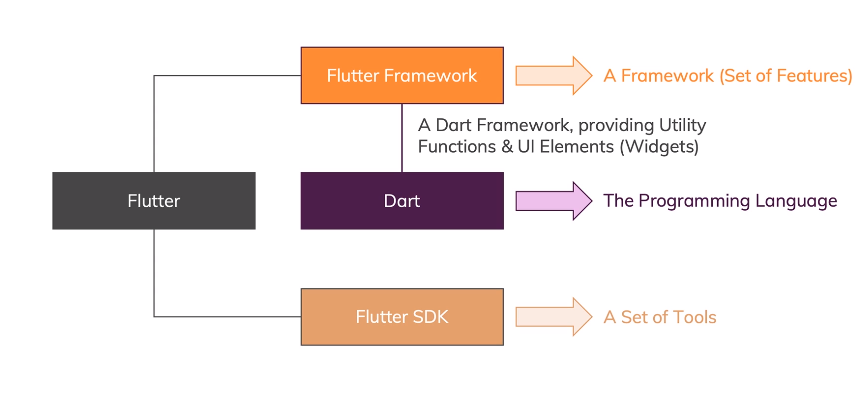
\includegraphics[width=9cm]{../libs/flutter-composition}
		\caption{Composizione Flutter}
		\label{fig: Composizione Flutter}
	\end{figure}
\end{frame}

%% ---------------------------------------------------------------------------

\begin{frame}{Dart}
	\begin{minipage}[0.2\textheight]{\textwidth}
		\begin{columns}[T]
			\begin{column}{0.4\textwidth}
				\begin{figure}[htpb]
					\centering
					
\includegraphics[width=4cm]{../libs/dart-logo.png}
					\caption{Dart logo}
					\label{fig:Dart logo}
				\end{figure}
			\end{column}
			\begin{column}{0.6\textwidth}
				\emph{Dart}
				\newline
				Dart è un linguaggio di programmazione sviluppato da Google.
				\begin{itemize}
					\item Finalizzato allo sviluppo frontend ed interfacce utente
					\item Fortemente tipizzato ed orientato agli oggetti
				\end{itemize}
			\end{column}
		\end{columns}
	\end{minipage}
\end{frame}

%% ---------------------------------------------------------------------------

\section{Flutter: Come}
\begin{frame}{Architettura}
	\begin{figure}[htpb]
		\centering
		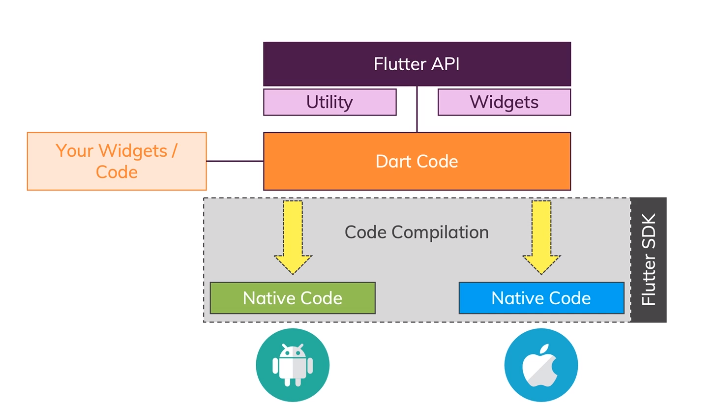
\includegraphics[width=9cm]{../libs/flutter-architecture}
		\caption{Architettura Flutter}
		\label{fig: Architettura Flutter}
	\end{figure}
\end{frame}

%% ---------------------------------------------------------------------------

\begin{frame}{Controllo totale di ogni pixel}
	\begin{minipage}[0.2\textheight]{\textwidth}
		\begin{columns}[T]
			\begin{column}{0.4\textwidth}
				\begin{figure}[htpb]
					\centering
					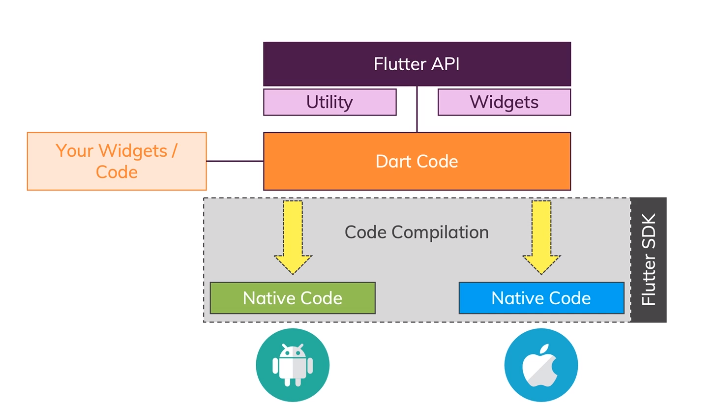
\includegraphics[width=4cm]{../libs/flutter-architecture}
					\caption{Architettura Flutter}
					\label{fig:Architettura Flutter}
				\end{figure}
			\end{column}
			\begin{column}{0.6\textwidth}
				\emph{Dart}
				\newline
				Flutter ha il controllo totale di ogni pixel disegnato
				\begin{itemize}
					\item Maggiore controllo
					\item Minore limitazioni date dalla piattaforme
					\item Migliori performance
				\end{itemize}
			\end{column}
		\end{columns}
	\end{minipage}
\end{frame}

%% ---------------------------------------------------------------------------

\begin{frame}{E' tutta una questione di widgets}
	\begin{figure}[htpb]
		\centering
		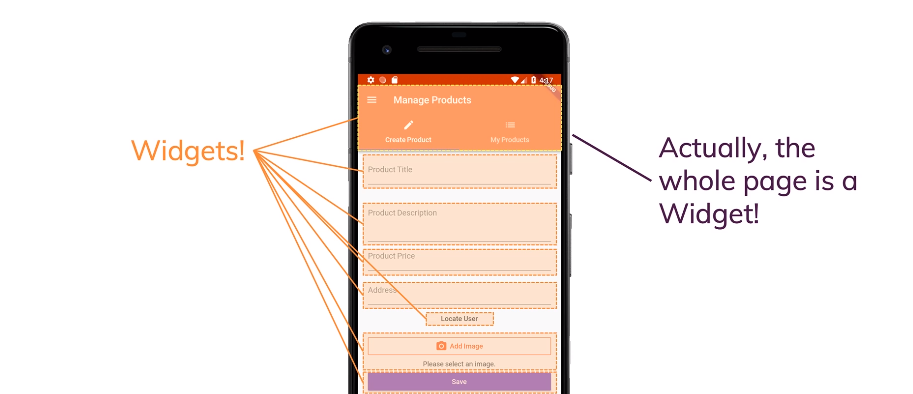
\includegraphics[width=9cm]{../libs/sample-widgets}
		\caption{Esempio widgets}
		\label{fig: Esempio widgets}
	\end{figure}
\end{frame}

%% ---------------------------------------------------------------------------

\begin{frame}{Composizione ad Albero}
	\begin{minipage}[0.2\textheight]{\textwidth}
		\begin{columns}[T]
			\begin{column}{0.5\textwidth}
				\begin{figure}[htpb]
					\centering
					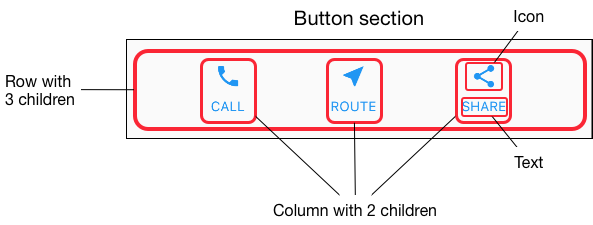
\includegraphics[width=4cm]{../libs/button-section-diagram}
					\caption{Esempio selezione \cite{flutterLayout}}
					\label{fig:Esempio selezione}
				\end{figure}
			\end{column}
			\begin{column}{0.5\textwidth}
				\begin{figure}[htpb]
					\centering
					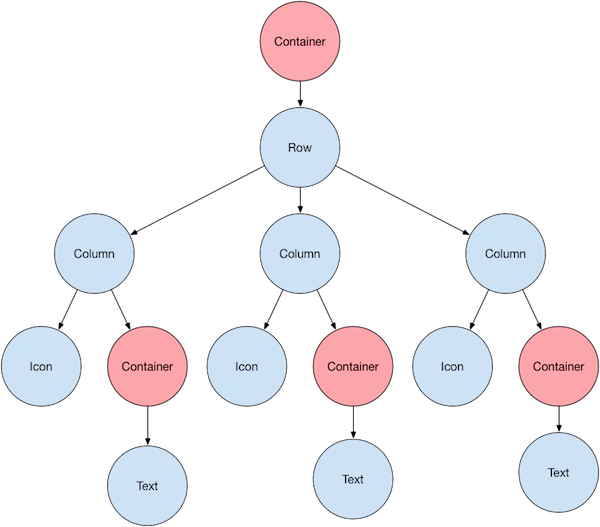
\includegraphics[width=4cm]{../libs/sample-flutter-layout}
					\caption{Esempio albero \cite{flutterLayout}}
					\label{fig:Esempio albero}
				\end{figure}
			\end{column}
		\end{columns}
	\end{minipage}
\end{frame}

%% ---------------------------------------------------------------------------

\section{Dart}
\begin{frame}{Prima di iniziare: DART!}
	\begin{minipage}[0.2\textheight]{\textwidth}
		\begin{columns}[T]
			\begin{column}{0.4\textwidth}
				\begin{figure}[htpb]
					\centering
					
\includegraphics[width=4cm]{../libs/dart-logo.png}
					\caption{Dart logo}
					\label{fig:Dart logo}
				\end{figure}
			\end{column}
			\begin{column}{0.6\textwidth}
				\emph{Giochiamo un po' con dart!}
				\newline
				\href{https://dartpad.dev/?}{\beamergotobutton{Lancia dart pad}}
			\end{column}
		\end{columns}
	\end{minipage}
\end{frame}

%% ---------------------------------------------------------------------------

% Reference frames
\begin{frame}[allowframebreaks]
    \frametitle{Riferimenti}
    \printbibliography
\end{frame}

%% ---------------------------------------------------------------------------
% Final frame
\section{Fine}
\begin{frame}{}
	\huge\emph{Grazie per l'attenzione!}
	\newline
	\vfill
	\hfill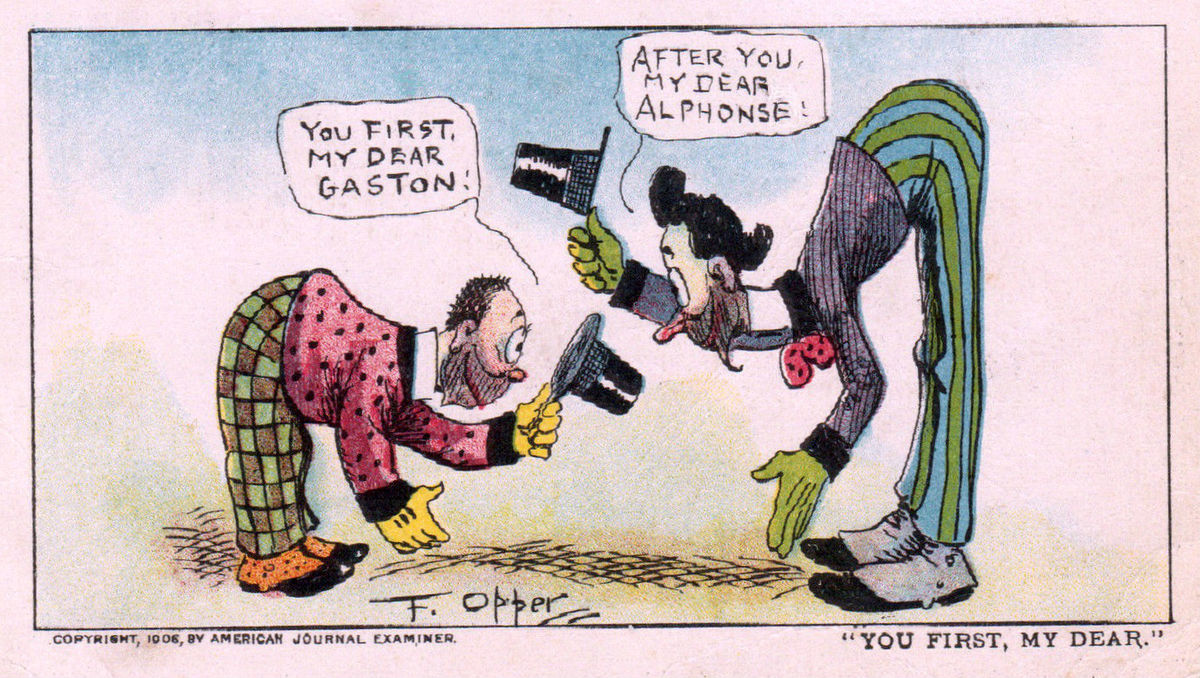
\includegraphics[width=6cm]{../libs/alphonse-gaston-regards}
\end{frame}

\end{document}